%!TEX TS-program = pdflatex
%!TEX encoding = UTF-8 Unicode
%!TEX spellcheck = English (Aspell)

\documentclass[11pt]{article}
\usepackage{lucy,handout,graphicx}

% =========================================================
\begin{document}

\headers{CSCI 332}{``Quiz 7'' group activity}{Fall 2026}


\noindent 
For each of the problems below, transform the input into a graph and apply a
standard graph algorithm that you’ve seen in class.
The first is given as an example.

Whenever you use a standard
graph algorithm, you \EMPH{must} provide the following information.  (I
recommend actually using a bulleted list.)
\begin{itemize}\itemsep0pt
\item What are the vertices?  What does each vertex represent?
\item What are the edges?  Are they directed or undirected?
\item If the vertices and/or edges have associated values, what are they?
\item \textbf{What is the precise relationship between your graph and the stated problem?}
\item What standard graph algorithm are you using to solve the problem?
\item What is the running time of your entire algorithm, \emph{including} the time to build the graph, \emph{as a function of the original input parameters}?
\end{itemize}
Finally, it is crucial to remember that even when you are explicitly given a graph as part of the input, that may not be the graph you actually want to search!

\bigskip
\hrule
\medskip

\begin{enumerate}
\parindent 1.5em \itemsep 2ex

%----------------------------------------------------------------------
\item 
A \EMPH{pixel map} is a two-dimensional array whose values represent colors;
the individual entries in the array are called \EMPH{pixels}, an abbreviation
of \emph{picture elements}. A \EMPH{connected region} in a pixel map is a
connected subset of pixels that all have the same color, where two pixels are
considered adjacent if they are immediate horizontal or vertical neighbors.
The \EMPH{flood fill} operation, commonly represented by a paint can in
raster-graphics editing software, changes every pixel in a connected region
to a new color; the input to the operation consists of the indices $i$ and $j$
of one pixel in the target region and the new color.

Describe and analyze an efficient algorithm for flood fill on an $n\times n$
pixel map.

\begin{center}
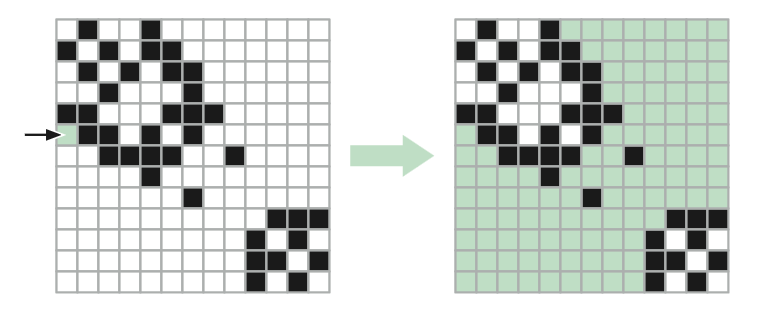
\includegraphics[width=0.85\linewidth]{floodfill.png}
\\
\footnotesize\sffamily
An example of flood fill.
\end{center}

\noindent\textbf{Solution.}
The flood-fill problem can be reduced to the reachability problem on a graph
$G$, which we describe below.
\begin{itemize}\itemsep2pt
\item What are the vertices?  What does each vertex represent?


The vertices are the individual pixels: one vertex for each entry in the
pixel map, regardless of its color.

\item What are the edges?  Are they directed or undirected?


The edges connect neighboring pixels with the same original color.
The edges are undirected, and neighbors are immediate horizontal or vertical
neighbors.

\item If the vertices and/or edges have associated values, what are they?


Each vertex has its pixel's color and array indices. The graph is unweighted;
no edge values are needed.

\item \textbf{What is the precise relationship between your graph and the stated problem?}


Each connected region in the pixel map is a component of $G$; thus, the
flood-fill problem reduces to a reachability problem in $G$.

\item What standard graph algorithm are you using to solve the problem?


Use whatever-first search in $G$, starting at the given pixel $(i,j)$, with
one minor modification: whenever we mark a vertex, we immediately change its
pixel's color to the new color. Build the graph before starting the search,
so recoloring pixels does not change its edges. The search marks exactly the
vertices in the starting pixel's component, so it recolors exactly the target
region.

\item What is the running time of your entire algorithm, \emph{including} the time to build the graph, \emph{as a function of the original input parameters}?


For an $n\times n$ pixel map, $G$ has $n^2$ vertices and at most $2n^2$
edges. Creating the vertices and checking each pixel's right and lower
neighbors to build the edges takes $O(n^2)$ time. Whatever-first search runs
in $O(|V|+|E|)=O(n^2)$ time, including constant time to recolor each marked
pixel. Thus the entire algorithm, including building the graph, takes
$O(n^2)$ time.
\end{itemize}



\item
A \EMPH{number maze} is an $n\times n$ grid of positive integers.  A token starts in the upper left corner; your goal is to move the token to the lower-right corner.  On each turn, you are allowed to move the token up, down, left, or right; the distance you may move the token is determined by the number on its current square.  For example, if the token is on a square labeled $3$, then you may move the token three steps up, three steps down, three steps left, or three steps right.  However, you are never allowed to move the token off the edge of the board.

\begin{center}
\footnotesize\sffamily
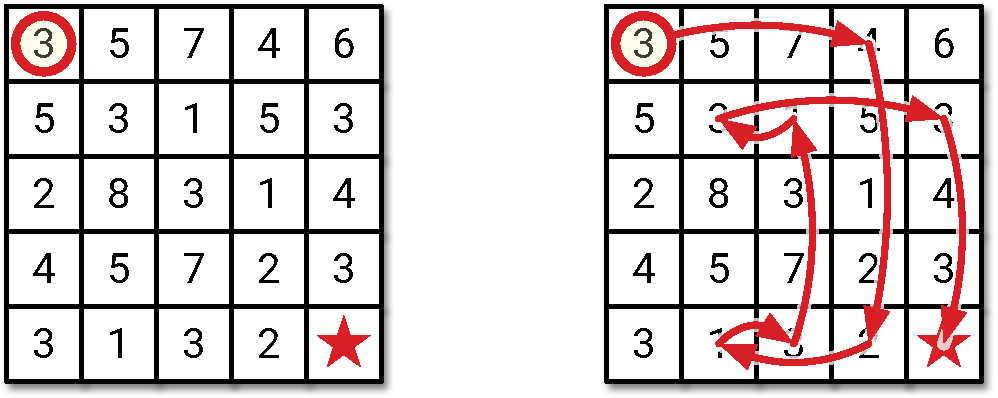
\includegraphics[scale=0.4]{numbermaze}
\\
A $5\times 5$ number maze that can be solved in eight moves.
\end{center}
%
Describe and analyze an efficient algorithm that either returns the minimum number of moves required to solve a given number maze, or correctly reports that the maze has no solution.  For example, given the number maze shown above, your algorithm should return the integer $8$.  Your input is a two-dimensional array $M[\range{1}{n}, \range{1}{n}]$ of positive integers.

\begin{itemize}\itemsep40pt
\item What are the vertices?  What does each vertex represent?
\item What are the edges?  Are they directed or undirected?
\item If the vertices and/or edges have associated values, what are they?
\item \textbf{What is the precise relationship between your graph and the stated problem?}
\item What standard graph algorithm are you using to solve the problem?
\item What is the running time of your entire algorithm, \emph{including} the time to build the graph, \emph{as a function of the original input parameters}?
\end{itemize}



The remaining problems consider variants of problem 2, where the sequence of moves must satisfy certain constraints to be considered a valid solution.  For each problem, your goal is to describe and analyze an algorithm that either returns the minimum number of moves in a \emph{valid} solution to a given number maze, or reports correctly that no valid solution exists.

%----------------------------------------------------------------------
\item
Suppose a sequence of moves is considered \emph{valid} if and only if the moves  alternate between horizontal and vertical.  That is, a valid move sequence never has two horizontal moves in a row or two vertical moves in a row.

Describe and analyze an algorithm that either returns the minimum number of moves in a valid solution to a given number maze, or reports correctly that no valid solution exists.


%----------------------------------------------------------------------
\item
Suppose a sequence of moves is considered \emph{valid} if and only if its length (the number of moves) is a multiple of $5$.

Describe and analyze an algorithm that either returns the minimum number of moves in a valid solution to a given number maze, or reports correctly that no valid solution exists.



\end{enumerate}



%----------------------------------------------------------------------


\end{document}